\documentclass[twoside,11pt]{article}

\usepackage{jmlr2e}
\usepackage{booktabs}
\usepackage{lastpage}
\usepackage{microtype}
\usepackage{url}
\hypersetup{hidelinks}

\newcommand{\pkg}{\texttt{fastEmbedR}}
\newcommand{\R}{\textsf{R}}

\jmlrheading{XX}{2026}{1--\pageref{LastPage}}{MM/YY}{MM/YY}{XX-0000}{Moussa Kassim, Martin Ocharo, Alessia Vignoli, Leonardo Tenori, and Stefano Cacciatore}
\ShortHeadings{Native UMAP and openTSNE for R}{Kassim, Ocharo, Vignoli, Tenori, and Cacciatore}
\firstpageno{1}

\begin{document}

\title{fastEmbedR: Native CPU, Metal, and CUDA Implementations of UMAP and openTSNE for R}

\author{\name Moussa Kassim$^{1,2}$ \email Moussa.Kassim@icgeb.org\\
\name Martin Ocharo$^{1,2}$ \email Martin.Ocharo@icgeb.org\\
\name Alessia Vignoli$^{3,4}$ \email vignoli@cerm.unifi.it\\
\name Leonardo Tenori$^{3,4}$ \email tenori@cerm.unifi.it\\
\name Stefano Cacciatore$^{1,2}$ \email stefano.cacciatore@icgeb.org\\
\addr $^1$Bioinformatics Unit, International Center for Genetic Engineering and Biotechnology,\\
Cape Town 7925, South Africa\\
$^2$Department of Integrative Biomedical Sciences, Institute of Infectious Disease \& Molecular Medicine (IDM),\\
University of Cape Town, Cape Town 7925, South Africa\\
$^3$Department of Chemistry ``Ugo Schiff'', University of Florence, Sesto Fiorentino, Italy\\
$^4$Magnetic Resonance Center (CERM), University of Florence, Sesto Fiorentino, Italy}

\editor{To be assigned}

\maketitle

\begin{abstract}%
The most widely used accelerated implementations of t-distributed stochastic neighbor embedding (t-SNE) and Uniform Manifold Approximation and Projection (UMAP) are fragmented across R, Python, C++, and accelerator-specific libraries. We present \pkg, an R package that implements complete UMAP and openTSNE-style t-SNE workflows with native CPU, Apple Metal, and NVIDIA CUDA execution. The package accepts either a data matrix or reusable nearest-neighbor indices and distances, constructs UMAP graphs or t-SNE affinities internally, and executes optimization without calling Python. Its numerical core uses compact float32 and int32 storage, while GPU paths retain major working arrays on device. Backend-native randomized PCA provides t-SNE initialization, and explicit landmark functions support reference embedding and projection of new observations. In three-seed HPC benchmarks across 11 image, cytometry, metabolomics, and single-cell datasets, nine datasets supported matched full-pipeline comparisons. Median speedups were 1.81-fold for four-thread CPU and 54.2-fold for CUDA openTSNE relative to Rtsne; fuzzy UMAP speedups were 1.31-fold for CPU and 63.5-fold for CUDA relative to uwot fast SGD. Median trustworthiness differences were $+0.039$, $+0.041$, $-0.0012$, and $-0.0012$, respectively. \pkg{} therefore makes accelerated embeddings directly available to R users through one coherent, inspectable API without concealing runtime or quality trade-offs.
\end{abstract}

\begin{keywords}
dimensionality reduction, t-SNE, UMAP, R software, GPU computing, Metal, CUDA
\end{keywords}

\section{Introduction}

t-SNE and UMAP are standard tools for high-dimensional biological and machine-learning data \citep{vandermaaten2008,mcinnes2018,kobak2019}. Barnes--Hut t-SNE, FIt-SNE, openTSNE, and GPU UMAP improved their scalability \citep{vandermaaten2014,linderman2019,policar2024,nolet2020}, but R users still encounter separate package interfaces, external executables, Python environments, and backend-specific data transfers. Moreover, a complete run includes neighbor search, affinity or graph construction, initialization, and iterative optimization; accelerating only one stage may not improve the user-visible call.

\pkg{} addresses this software gap with one R interface backed by native CPU, Apple Metal, and NVIDIA CUDA implementations. It is not a wrapper around Python openTSNE or RAPIDS cuML. The package owns KNN-to-affinity/graph conversion, initialization, sparse schedules, optimization state, landmark projection, return objects, timing metadata, and backend validation. Optional platform libraries provide narrowly defined primitives such as CUDA search, truncated SVD, or FFTs. The resulting public API supports both complete matrix-input workflows and direct reuse of precomputed KNN matrices.

\section{Software Architecture and Implementations}

\subsection{R interface and computational boundary}

The matrix-input functions \texttt{opentsne()} and \texttt{umap()} accept ordinary R matrices. They also accept float32 matrices from the \texttt{float} package. The KNN-entry functions, \path{opentsne_knn()} and \path{umap_knn()}, accept reusable integer neighbor indices and floating-point distances. Backend selection is explicit: \texttt{backend="cpu"}, \texttt{"metal"}, or \texttt{"cuda"}. An unavailable GPU request fails rather than silently running on CPU.

For matrix input, CPU neighbor search uses a package-resident HNSW implementation distilled from permissively licensed FAISS code \citep{johnson2019,douze2024}; Metal uses native exact or recall-tuned IVF-Flat kernels; CUDA links to installed FAISS GPU exact search or the cuVS IVF-Flat C API and can keep KNN buffers on the device. The source distributions of these libraries are not vendored. The exported \texttt{pca()} function uses randomized/truncated SVD \citep{halko2011}: CPU follows the \texttt{fastPLS} RSVD design, Metal uses a native float32 block-subspace method with MPS products, and CUDA uses RAFT TSVD. Setting \texttt{opentsne\_init=TRUE} returns the small-scale PCA initialization used by modern t-SNE practice \citep{kobak2019,fastpls}.

The portable core is compiled as C++17 and adds only POSIX-thread linkage to the flags selected by the active R installation. Metal builds link the Apple Metal/MPS frameworks; CUDA builds use C++17 NVCC translation units with explicit deployment architectures and an R-ABI-compatible host compiler. The package does not impose global \texttt{-march=native}, \texttt{-ffast-math}, or \texttt{-O3}; exact resolved flags and dependency architectures are recorded with each reproducibility bundle.

\subsection{Native UMAP}

Fuzzy UMAP estimates per-row $\rho_i$ and $\sigma_i$, forms directed memberships, and combines reciprocal edges as $w_{ij}+w_{ji}-w_{ij}w_{ji}$ \citep{mcinnes2018}. The explicit \texttt{graph\_mode="binary"} alternative uses the symmetric KNN union with unit weights and is reported as an approximation. Both modes use the package's low-dimensional attraction/repulsion, negative sampling, learning-rate decay, and size-aware epoch policy.

The graph is stored once as CSR int32 offsets/indices plus float32 weights and edge schedules. CPU code parallelizes row-wise bandwidth estimation, graph construction, sparse initialization products, and edge updates. Metal uploads the schedule once and keeps coordinates and optimizer state in unified GPU memory. CUDA can consume GPU-resident KNN buffers, prepare the graph on-device, and execute the package-native atomic optimizer. \texttt{uwot} is a behavioral benchmark, not a source or runtime dependency \citep{uwot}.

\subsection{Native openTSNE-style t-SNE}

\texttt{opentsne\_knn()} obtains row-conditional Gaussian probabilities by perplexity-matched bandwidth search, then symmetrizes and normalizes sparse affinities. Its two phases implement early exaggeration and normal optimization with automatic learning rates, gains, momentum, clipping, recentering, sparse attractive forces, and exact or interpolation-grid negative gradients \citep{vandermaaten2008,linderman2019,policar2024,belkina2019}. No openTSNE Python/Cython code is called.

CPU execution reuses FFT plans, interpolation grids, and worker scratch. Metal performs grid scatter, package-native two-dimensional FFT convolution, interpolation, sparse attraction, and updates in Metal kernels; its validated $512\times512$ Stockham transform follows permissively licensed Apple GPU design ideas \citep{applesiliconfft}. CUDA retains affinities, coordinates, gains, updates, cuFFT plans, and grids on-device and groups repeated iterations with CUDA Graph execution. This sparse-attraction/interpolated-repulsion organization follows FIt-SNE and t-SNE-CUDA without invoking their executables \citep{linderman2019,chan2018}.

\subsection{Precision and scalable transforms}

Working data, distances, weights, coordinates, gradients, gains, and workspaces use float32; graph indices use int32. Float32 R input avoids an initial double conversion and receives a float32 layout, although total process memory also includes R objects, indices, FFT grids, and library workspaces. \texttt{landmark\_tsne()} and \texttt{landmark\_umap()} embed a reference subset, interpolate remaining observations, apply a local affine correction, and optionally refine projected points. The t-SNE transform holds reference coordinates fixed as in \citet{policar2021}; the result records the approximation and each timing component. Detailed equations and dependency ownership are in the supplement.

\section{Evaluation}

We evaluated 11 datasets spanning 873 to 5,220,347 observations and 11 to 16,384 variables. Each method was run with seeds 4, 17, and 42; $k=30$ or perplexity 30; four requested CPU threads or one CUDA device; and its documented production optimizer. Competing methods on a machine used the same R environment, compiler toolchain, and thread controls. Cross-package comparisons report total public-function time because reference implementations expose different boundaries; KNN and initialization are not subtracted. Labels are used only for post hoc metrics \citep{venna2001,rousseeuw1987}. Figures~\ref{fig:hpcquality} and~\ref{fig:datasets} show representative results; complete timings, memory, quality, parameters, failures, compiler configuration, and Python/RAPIDS comparisons are supplied in the supplement.

On MNIST70k, median total times were 69.56 and 1.94 seconds for CPU/CUDA openTSNE versus 125.83 seconds for Rtsne, and 50.04 and 0.99 seconds for CPU/CUDA fuzzy UMAP versus 65.34 seconds for uwot fast SGD. Across nine matched datasets, median speedups were 1.81 and 54.2 for CPU/CUDA openTSNE and 1.31 and 63.5 for CPU/CUDA fuzzy UMAP. Corresponding median trustworthiness differences were $+0.039$, $+0.041$, $-0.0012$, and $-0.0012$; median Preserve@30 differences for fuzzy UMAP were $-0.0013$ and $-0.0024$. CPU peak-RSS ratios were 0.81 versus Rtsne and 0.63 versus uwot. Matched claims exclude unavailable or failed rows.

Correctness was evaluated at the mathematical boundaries. On a 2,000-point MNIST validation, t-SNE affinity edge Jaccard was 1.000, weight Pearson correlation was 1.000, and weight Spearman correlation was 0.852 against Python openTSNE. The fuzzy UMAP graph shared all validated edges with \texttt{uwot::similarity\_graph}; common-edge weight Pearson and Spearman correlations were 0.99999 and 0.99998. Across three MNIST seeds, openTSNE CPU/CUDA Procrustes correlations exceeded 0.9993 and neighbor stability@15 ranged from 0.929 to 0.953. These tests support behavioral equivalence without claiming bitwise identity.

\section{Discussion and Availability}

\pkg{} exposes established t-SNE and UMAP objectives consistently across multicore CPU, Metal, and CUDA, with matrix/KNN inputs, float32 storage, backend-native PCA, and reference transforms. FAISS, cuVS, RAFT, cuFFT, and MPS provide optional primitives; affinity/graph construction and embedding optimization remain package code. A complete analysis stays in R: one-call functions include search and initialization, while KNN-entry functions expose a controlled reusable boundary and both routes share the same builders and optimizers.

Correctness is assessed behaviorally because stochastic embeddings need not have identical coordinates. Fixed seeds control sampling and initialization, although atomic GPU summation order can vary. Landmark functions embed an explicit reference subset, initialize remaining points by interpolation and local affine correction, and optionally refine them against the fixed reference; component timings keep the approximation visible.

Speed depends on hardware, dimension, KNN recall, connectivity, and initialization. Binary UMAP is an explicit approximation and fuzzy mode the standard comparison. Landmarking is not uniformly faster: on MNIST CPU, 50\% landmark binary UMAP was 1.10-fold faster with trustworthiness changing by $-0.0010$, whereas landmark openTSNE was slower; failed CUDA landmark rows support no speed claim. \pkg{} is MIT licensed at \url{https://github.com/tkcaccia/fastEmbedR}; the repository provides installation guidance, tests, benchmarks, and generated benchmark tables. A clean release commit and archival DOI will be frozen before submission.

\clearpage

\begin{figure}[p]
\centering
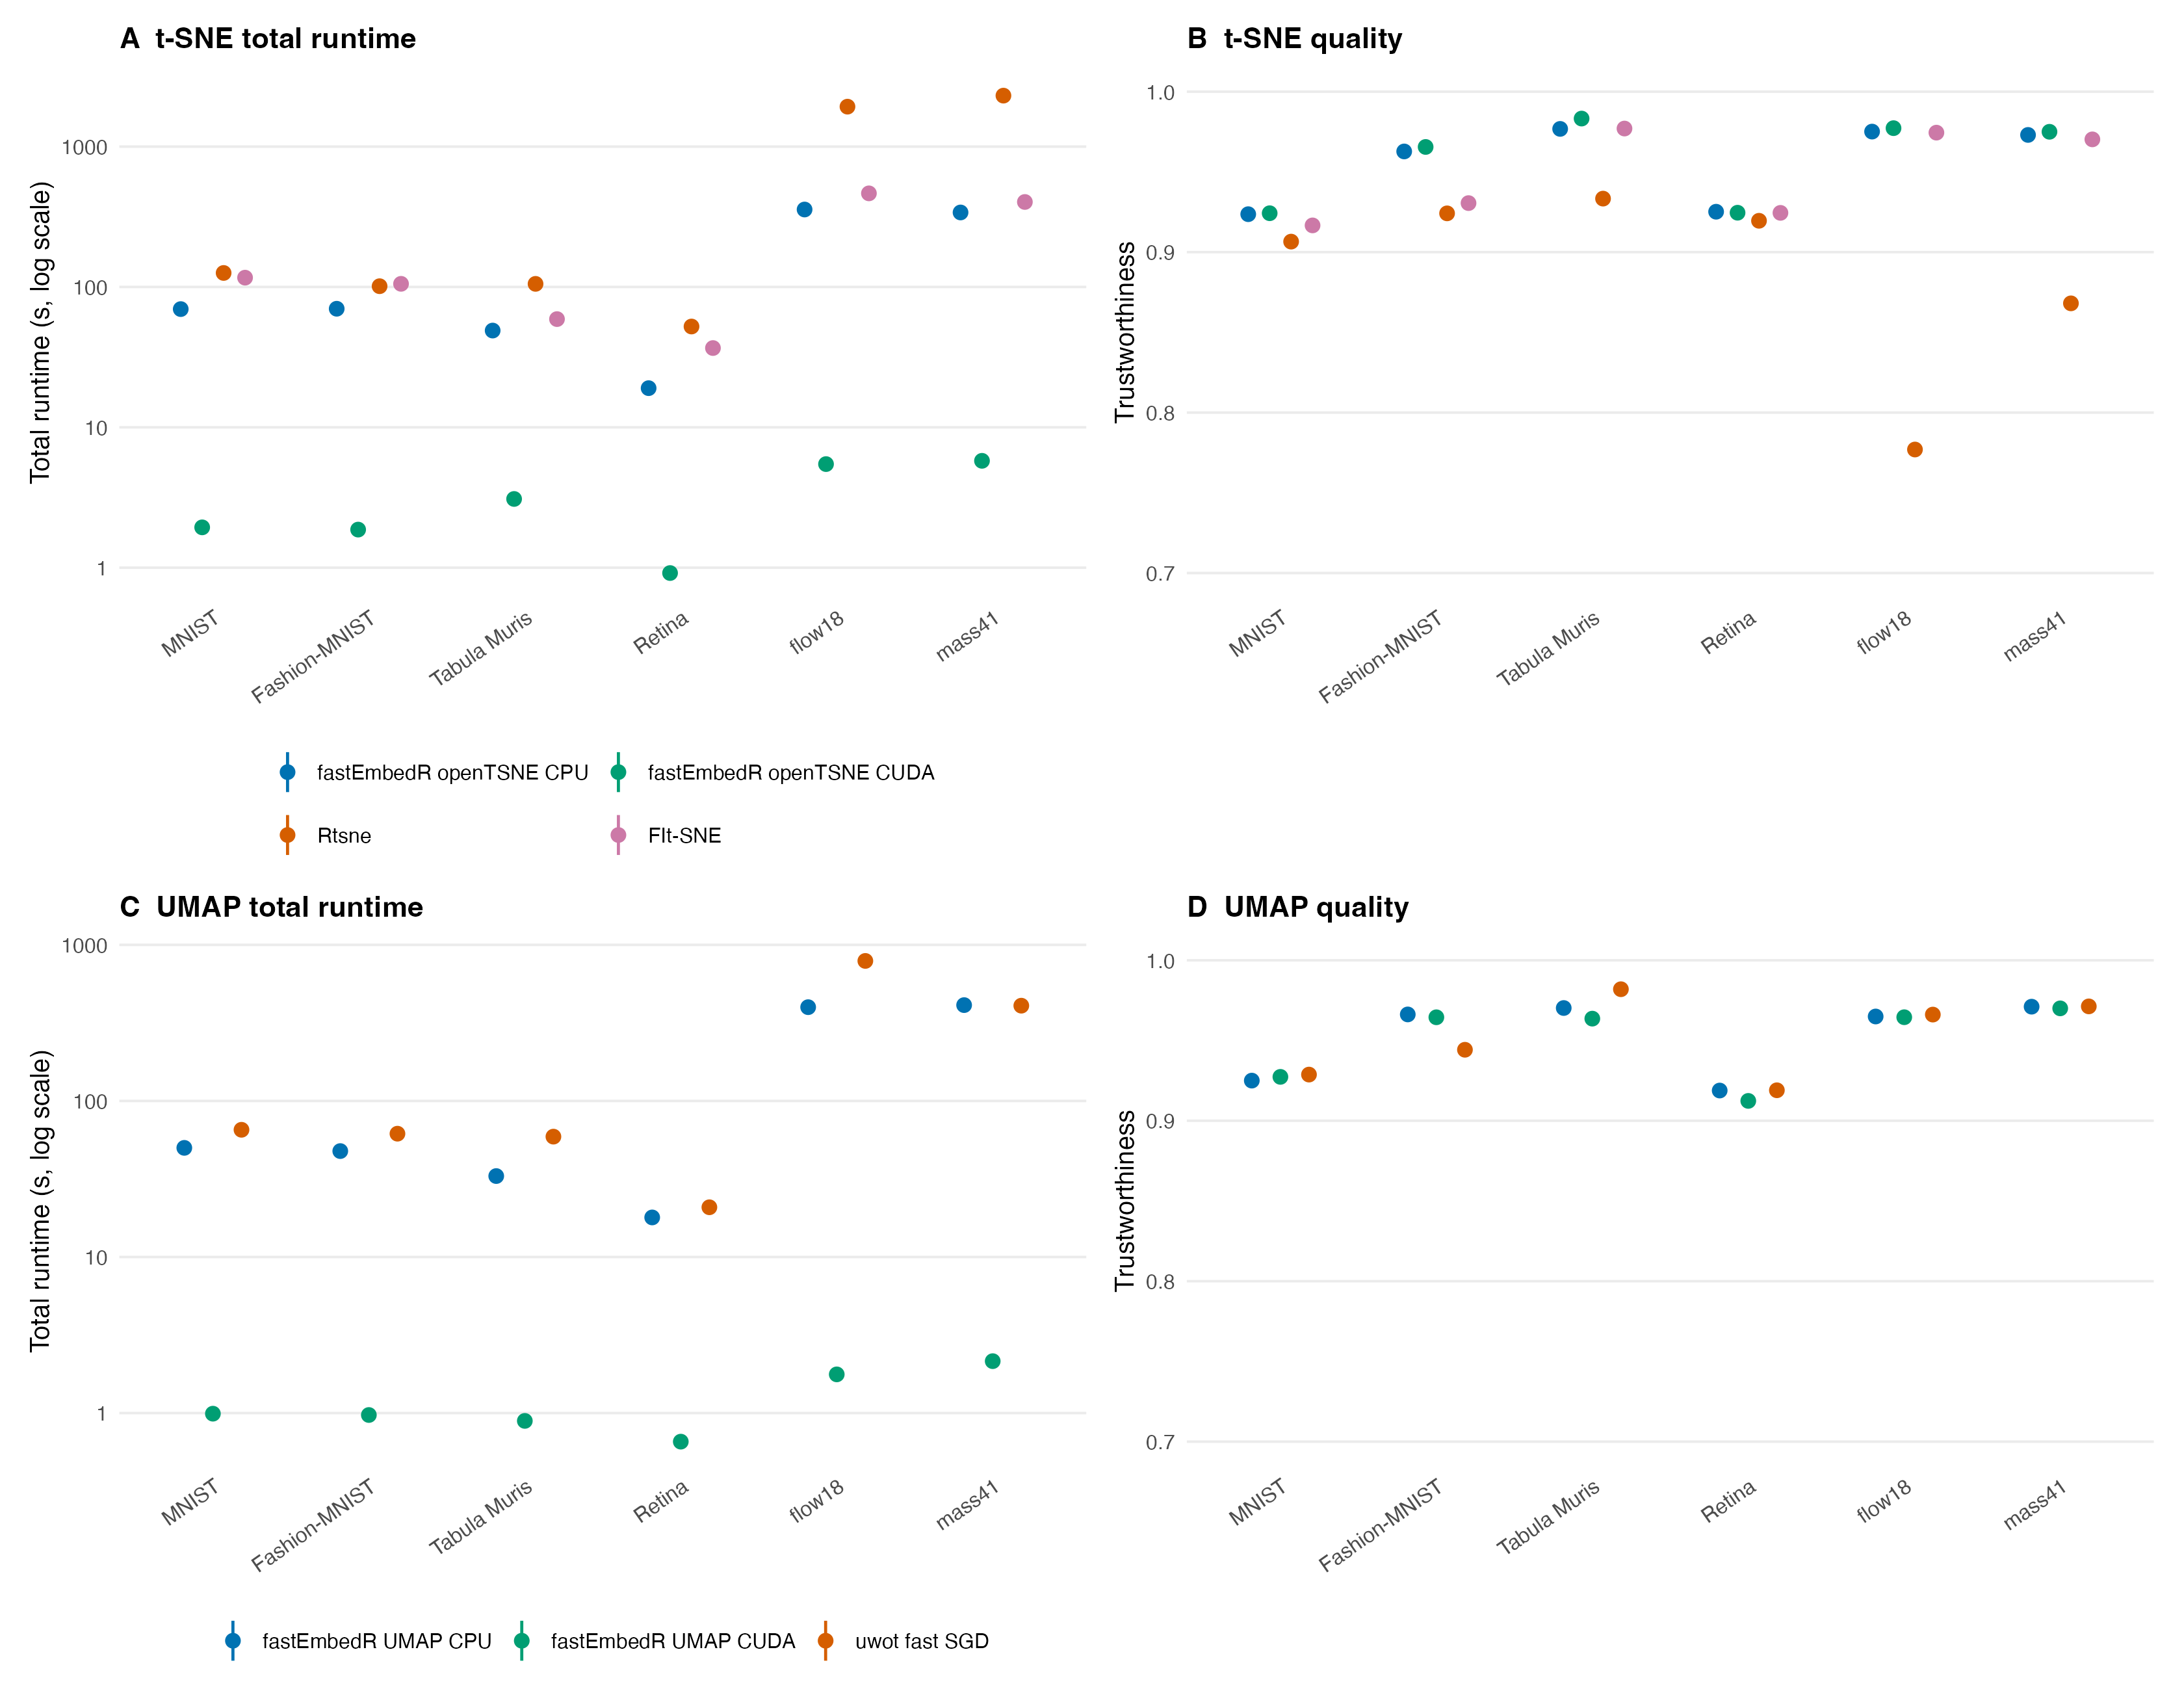
\includegraphics[width=\textwidth]{figures/hpc_runtime_quality.png}
\caption{Runtime and quality on six representative HPC datasets. Points are medians over seeds 4, 17, and 42; runtime bars span the interquartile range and use a logarithmic axis. CPU methods requested four threads. Labels were used only for post hoc metrics.}
\label{fig:hpcquality}
\end{figure}

\clearpage

\begin{figure}[p]
\centering
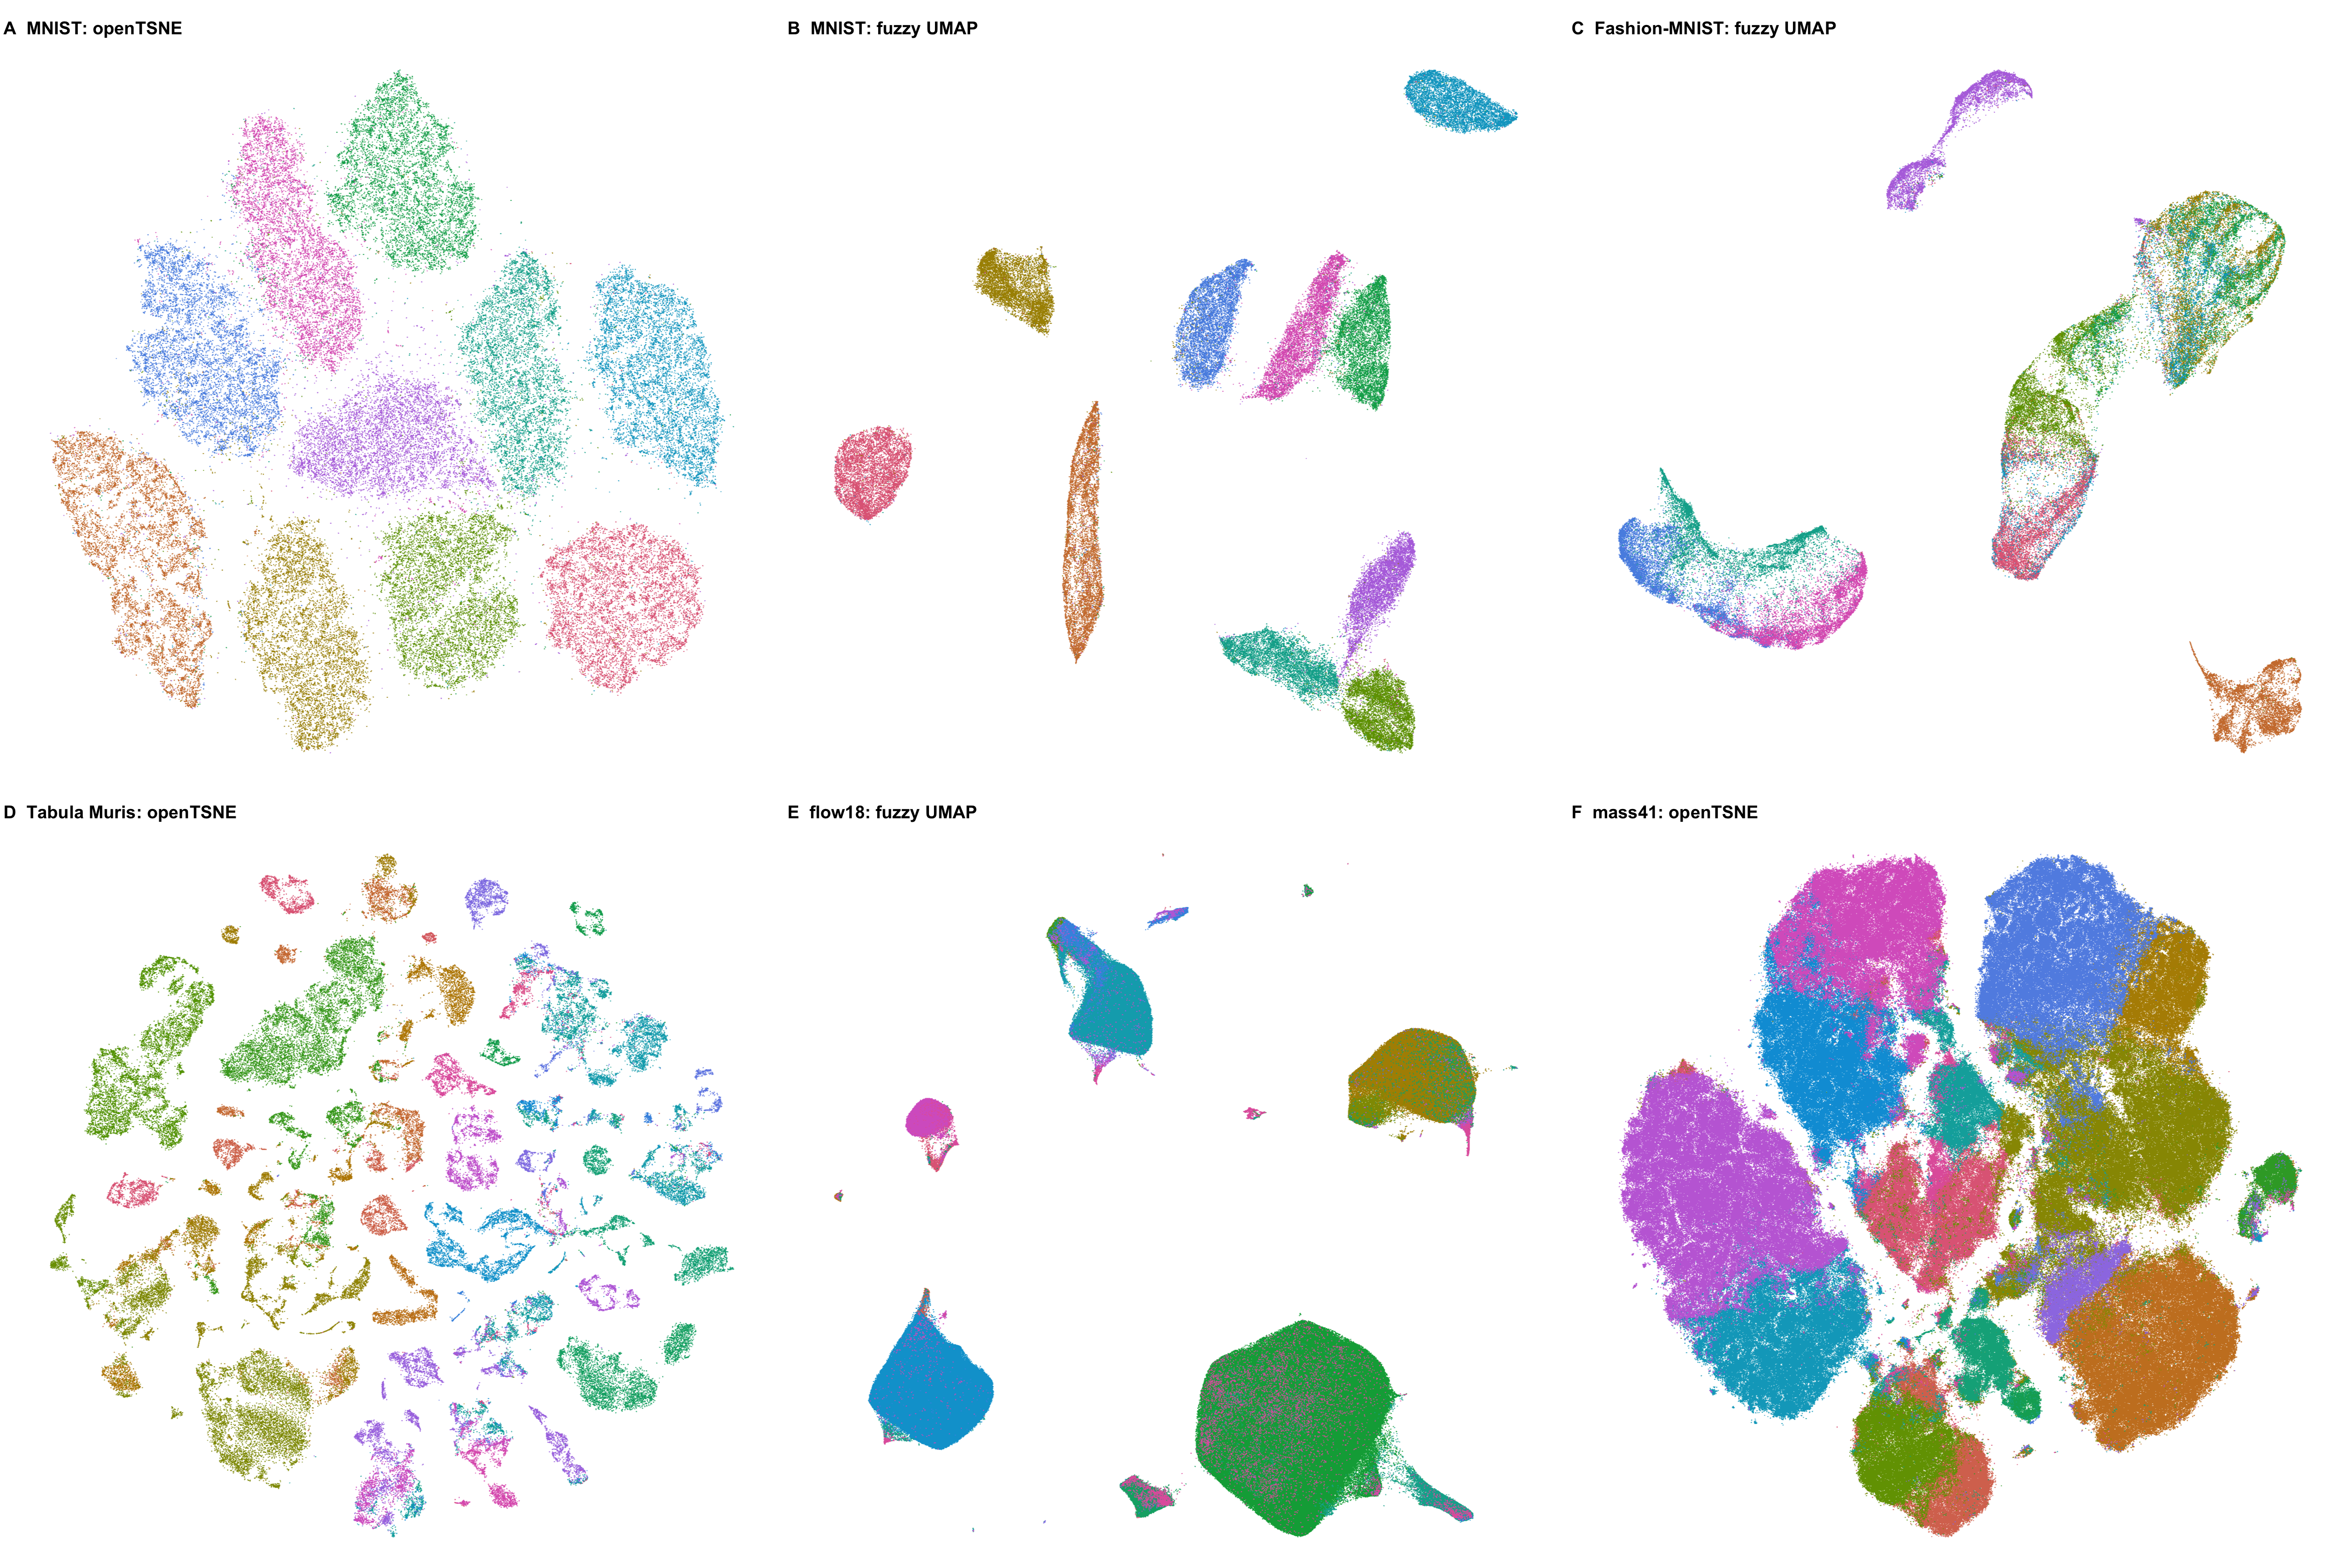
\includegraphics[width=\textwidth]{figures/hpc_representative_embeddings.png}
\caption{Representative label-colored CUDA embeddings from the archived HPC benchmark (seed 4). Labels were not supplied during fitting. Panels illustrate image, single-cell transcriptomic, flow-cytometry, and mass-cytometry inputs; plotting uses points only, without axes or boxes.}
\label{fig:datasets}
\end{figure}

\clearpage
\bibliography{fastEmbedR_MLOSS}

\end{document}
